\documentclass[pdftex,12pt,a4paper]{article}

\usepackage[turkish,english]{}
\usepackage{graphicx}  
\usepackage[margin=2.5cm]{geometry}
\usepackage{breakcites}
\usepackage{indentfirst}
\usepackage{pgfgantt}
\usepackage{pdflscape}
\usepackage{float}
\usepackage{epsfig}
\usepackage{epstopdf}
\usepackage[cmex10]{amsmath}
\usepackage{url}
\usepackage{stfloats}
\usepackage{multirow}
% \usepackage{karnaugh-map}

\newcommand*\andOp{{\mkern 2mu\cdot\mkern 2mu}}
\renewcommand{\refname}{REFERENCES}

\linespread{1.3}

\usepackage{mathtools}
%\newcommand{\HRule}{\rule{\linewidth}{0.5mm}}
\thispagestyle{empty}
\begin{document}
\begin{titlepage}
\begin{center}
\textbf{}\\
\textbf{\Large{ISTANBUL TECHNICAL UNIVERSITY}}\\
\vspace{0.5cm}
\textbf{\Large{COMPUTER ENGINEERING DEPARTMENT}}\\
\vspace{2cm}
\textbf{\Large{BLG 242E\\ DIGITAL CIRCUITS LABORATORY\\ EXPERIMENT REPORT}}\\
\vspace{2.8cm}
\begin{table}[ht]
\centering
\Large{
\begin{tabular}{lcl}
\textbf{EXPERIMENT NO}  & : & 2 \\
\textbf{EXPERIMENT DATE}  & : & 22.02.2019 \\
\textbf{LAB SESSION}  & : & FRIDAY - 14.00 \\
\textbf{GROUP NO}  & : & G13 \\
\end{tabular}}
\end{table}
\vspace{1cm}
\textbf{\Large{GROUP MEMBERS:}}\\
\begin{table}[ht]
\centering
\Large{
\begin{tabular}{rcl}
{
150180704  & : & C\.{I}HAT AKK\.{I}RAZ \\
150180707  & : & FAT\.{I}H ALTINPINAR \\
150180734  & : & S\.{I}NAN \c{S}AR \\
}
\end{tabular}}
\end{table}
\vspace{2.8cm}
\textbf{\Large{SPRING 2019}}

\end{center}

\end{titlepage}

\newpage

\thispagestyle{empty}
\centering{\LARGE{ \textbf{ETHIC FORM}}}\\
\centering{\LARGE{\textbf{for}}}\\
\centering{\LARGE{\textbf{BLG242E Logic Circuits Laboratory}}}\\[0.2cm]
As a student of \\Istanbul Technical University Faculty of Computer and Informatics Engineering;
\begin{enumerate}
    \item I will not attempt to cheat in quizes and final exam,
    \item I will not use disallowed sources or tools (mobile phone, calculator etc.) during the exam,
    \item I will not write any information (formula, text, figure etc.) on the table, sheets or books that are allowed to be used during the exam,
    \item I will give reference when using printed or online published sources,
    \item I will not use the results in a source as they are, or by changing a part of them without giving a reference,
    \item I will not show unused sources as used, 
    \item I will not present someone else’s idea as my own idea, 
    \item I will not make someone do my homework, project or thesis for money or anything else,
    \item I will not take an exam or enter a lecture on behalf of others,
    \item I will not make excuses for not attending in exams or lessons by taking reports from someone I know (medical doctor parents or relatives),
    \item I will refrain from deliberately harming the public materials at our university,  
    \item I will comply with the safety rules in laboratory work,
    \item I will behave in accordance with the rules of respect for the lecturers and teaching assistants
\end{enumerate}
\vspace{-1em}
\centering{\LARGE{signed by}}\\
\vspace{-1em}
\begin{table}[ht]
\centering
\begin{tabular}{rcl}
150180704  & : & C\.{I}HAT AKK\.{I}RAZ \\
150180707  & : & FAT\.{I}H ALTINPINAR \\
150180734  & : & S\.{I}NAN \c{S}AR \\
\end{tabular}
\end{table}
\vspace{-1em}
 \begin{table}[ht]
 \begin{tabular}{lr}
%\textbf{Date:\hspace*{1.0cm}/\hspace*{1.0cm}/} &\qquad \qquad\qquad\qquad \qquad\qquad\qquad \qquad\qquad\qquad \qquad\qquad \textbf{SIGNED}\\
\end{tabular}
\end{table} % adds the ethic sign
\addcontentsline{toc}{section}{\numberline {}ETHICS}
\newpage

\thispagestyle{empty}
\addtocontents{toc}{\contentsline {section}{\numberline {}FRONT COVER}{}}
\addtocontents{toc}{\contentsline {section}{\numberline {}CONTENTS}{}}
\setcounter{tocdepth}{4}
\tableofcontents
\clearpage

%\begin{figure}[ht]
%	\centering
%	\includegraphics[width=0.5\textwidth]{log%o.png}	
%	\caption{Figure 1}
%	\label{fig1}
%\end{figure}

\setcounter{page}{1}
\section{INTRODUCTION }
\begin{flushleft}
\paragraph{} 
% uzatma simulator xd  satış bitti!!
In this experiment we created truth tables for given functions then we implemented each and every function. We have compared our expected results to the outputs of the circuits we have built in order to prove given theorems or check our calculations.
% nice la xd cince guzel demek abi  herhalde dotada bagiriyorlardi burdan % chatlesmek de guzelasdaskda;sd 
\end{flushleft}
  

\section{REQUIREMENTS}

\begin{flushleft}
\underline{Tools Used}\cite{booklet}
\end{flushleft}
\begin{itemize}
    \item C.A.D.E.T
    \item 74000 series ICs
    \begin{itemize}
        \item 74x$x^{1}$04 - Hex Inverter
        \item 74x$x^{1}$08 - Quadruple 2-input Positive AND Gates
        \item 74x$x^{1}$32 - Quadruple 2-input Positive OR Gates
    \end{itemize}
\end{itemize}


\begin{flushleft}
\subsection{PART 1}

\paragraph{}
In the first part of the experiment, the logic circuits are designed and implemented for the given expressions below.

\begin{itemize}
    \item $F_{1}$(a,b) = a + $a \cdot b$
    \item $F_{2}$(a,b) = $(a + b) \cdot (a + b')$
\end{itemize}

\paragraph{}
First of all, truth tables are created for these expressions.


\begin{table}[h]
    \centering
    \begin{tabular}{|c|c|c|c|}
    \hline
    a & b & $a \cdot b$ & a + $a \cdot b$ \\ \hline
    0 & 0 & 0     & 0         \\
    0 & 1 & 0     & 0         \\
    1 & 0 & 0     & 1         \\
    1 & 1 & 1     & 1         \\ \hline
    \end{tabular}
    \caption{Truth table of $F_1$}
    \label{fig1}
\end{table}

\newpage

\begin{table}[!h]
    \centering
    \begin{tabular}{|c|c|c|c|c|c|}
    \hline
    a & b & b' & a + b & a + b' & $(a + b) \cdot (a + b')$ \\ \hline
    0 & 0 & 1  & 0     & 1      & 0                  \\
    0 & 1 & 0  & 1     & 0      & 0                  \\
    1 & 0 & 1  & 1     & 1      & 1                  \\
    1 & 1 & 0  & 1     & 1      & 1                  \\ \hline
    \end{tabular}
    \caption{Truth table of $F_2$}
    \label{fig2}
\end{table}



\begin{figure}[!h]
	\centering
	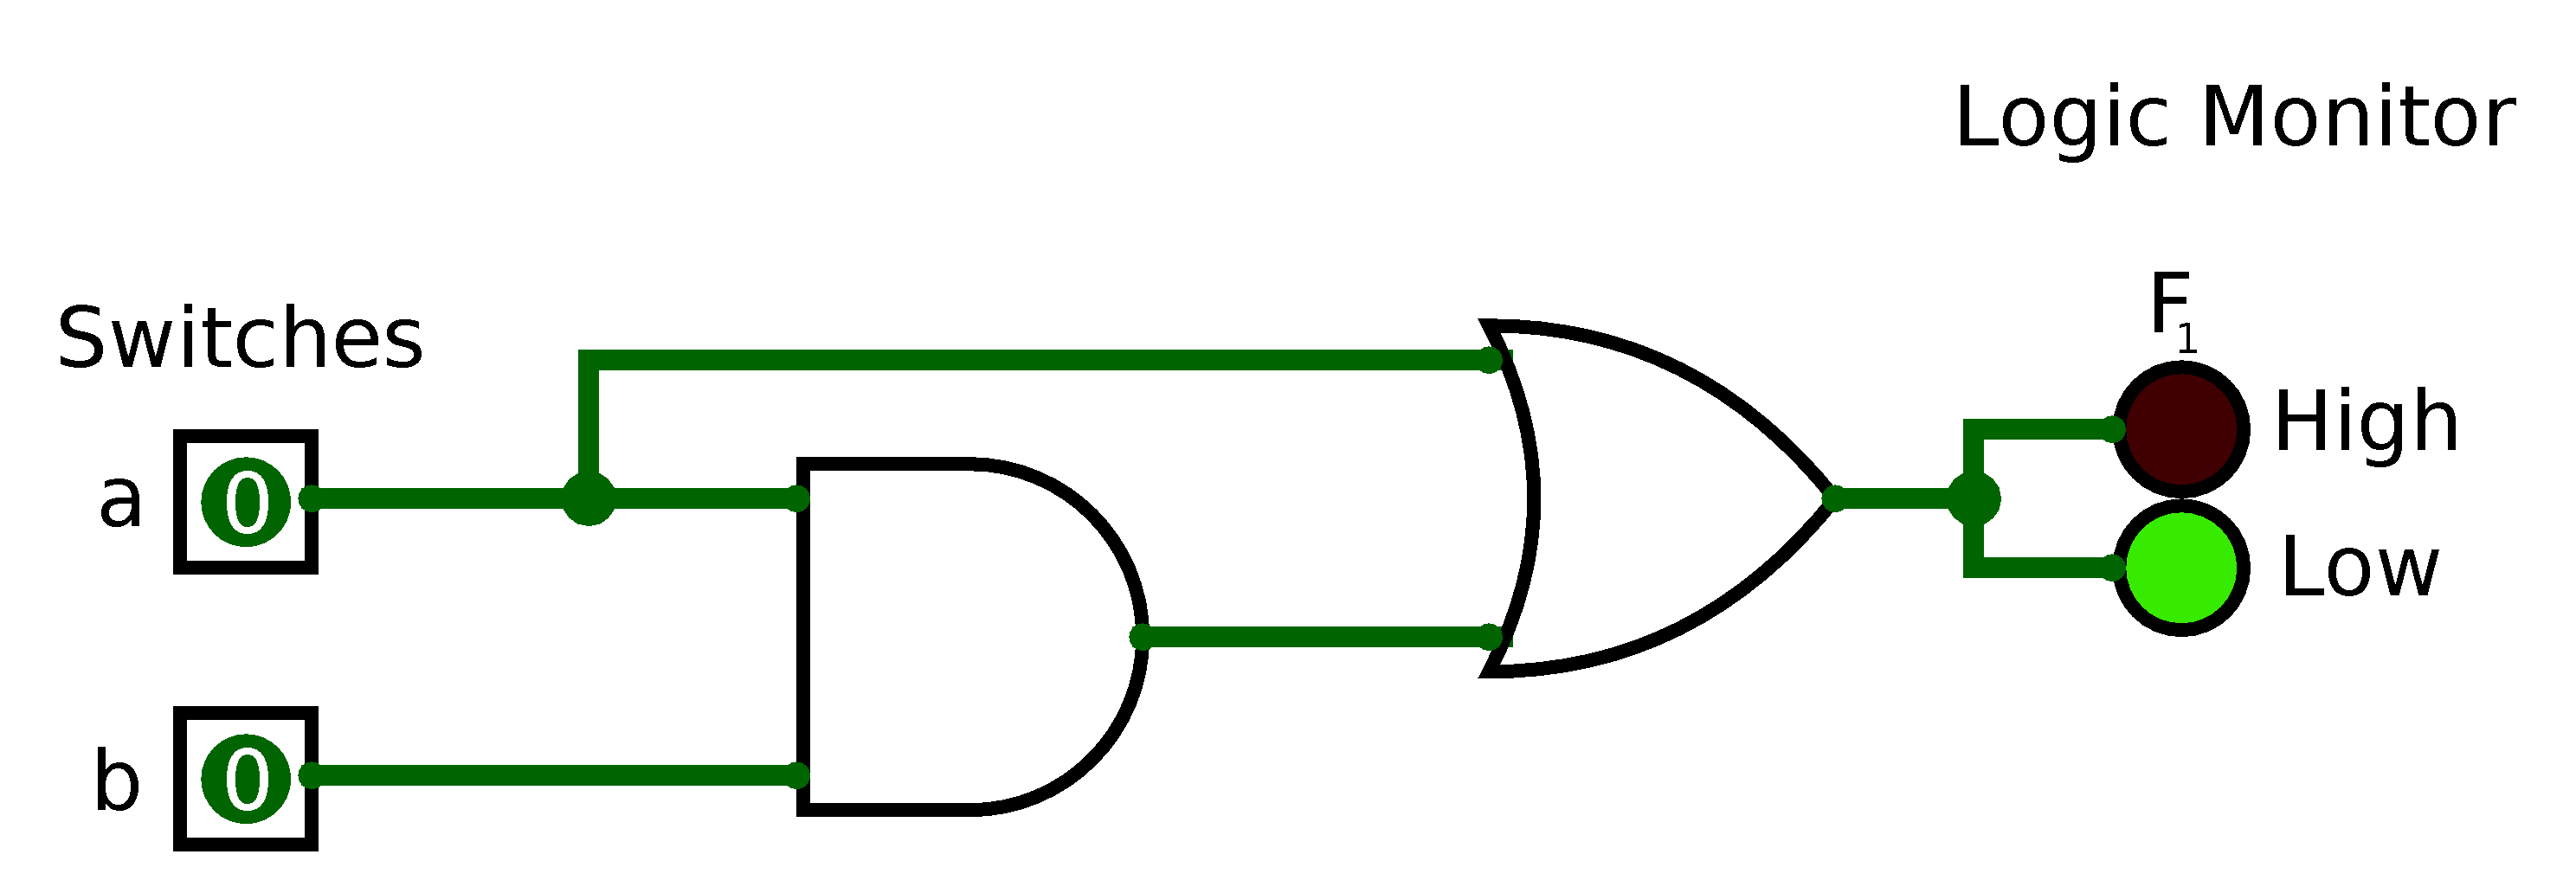
\includegraphics[width=0.5\textwidth]{part1-f1.png}	
	\caption{Circuit of $F_1$}
	\label{fig1}
\end{figure}


\begin{figure}[!h]
	\centering
	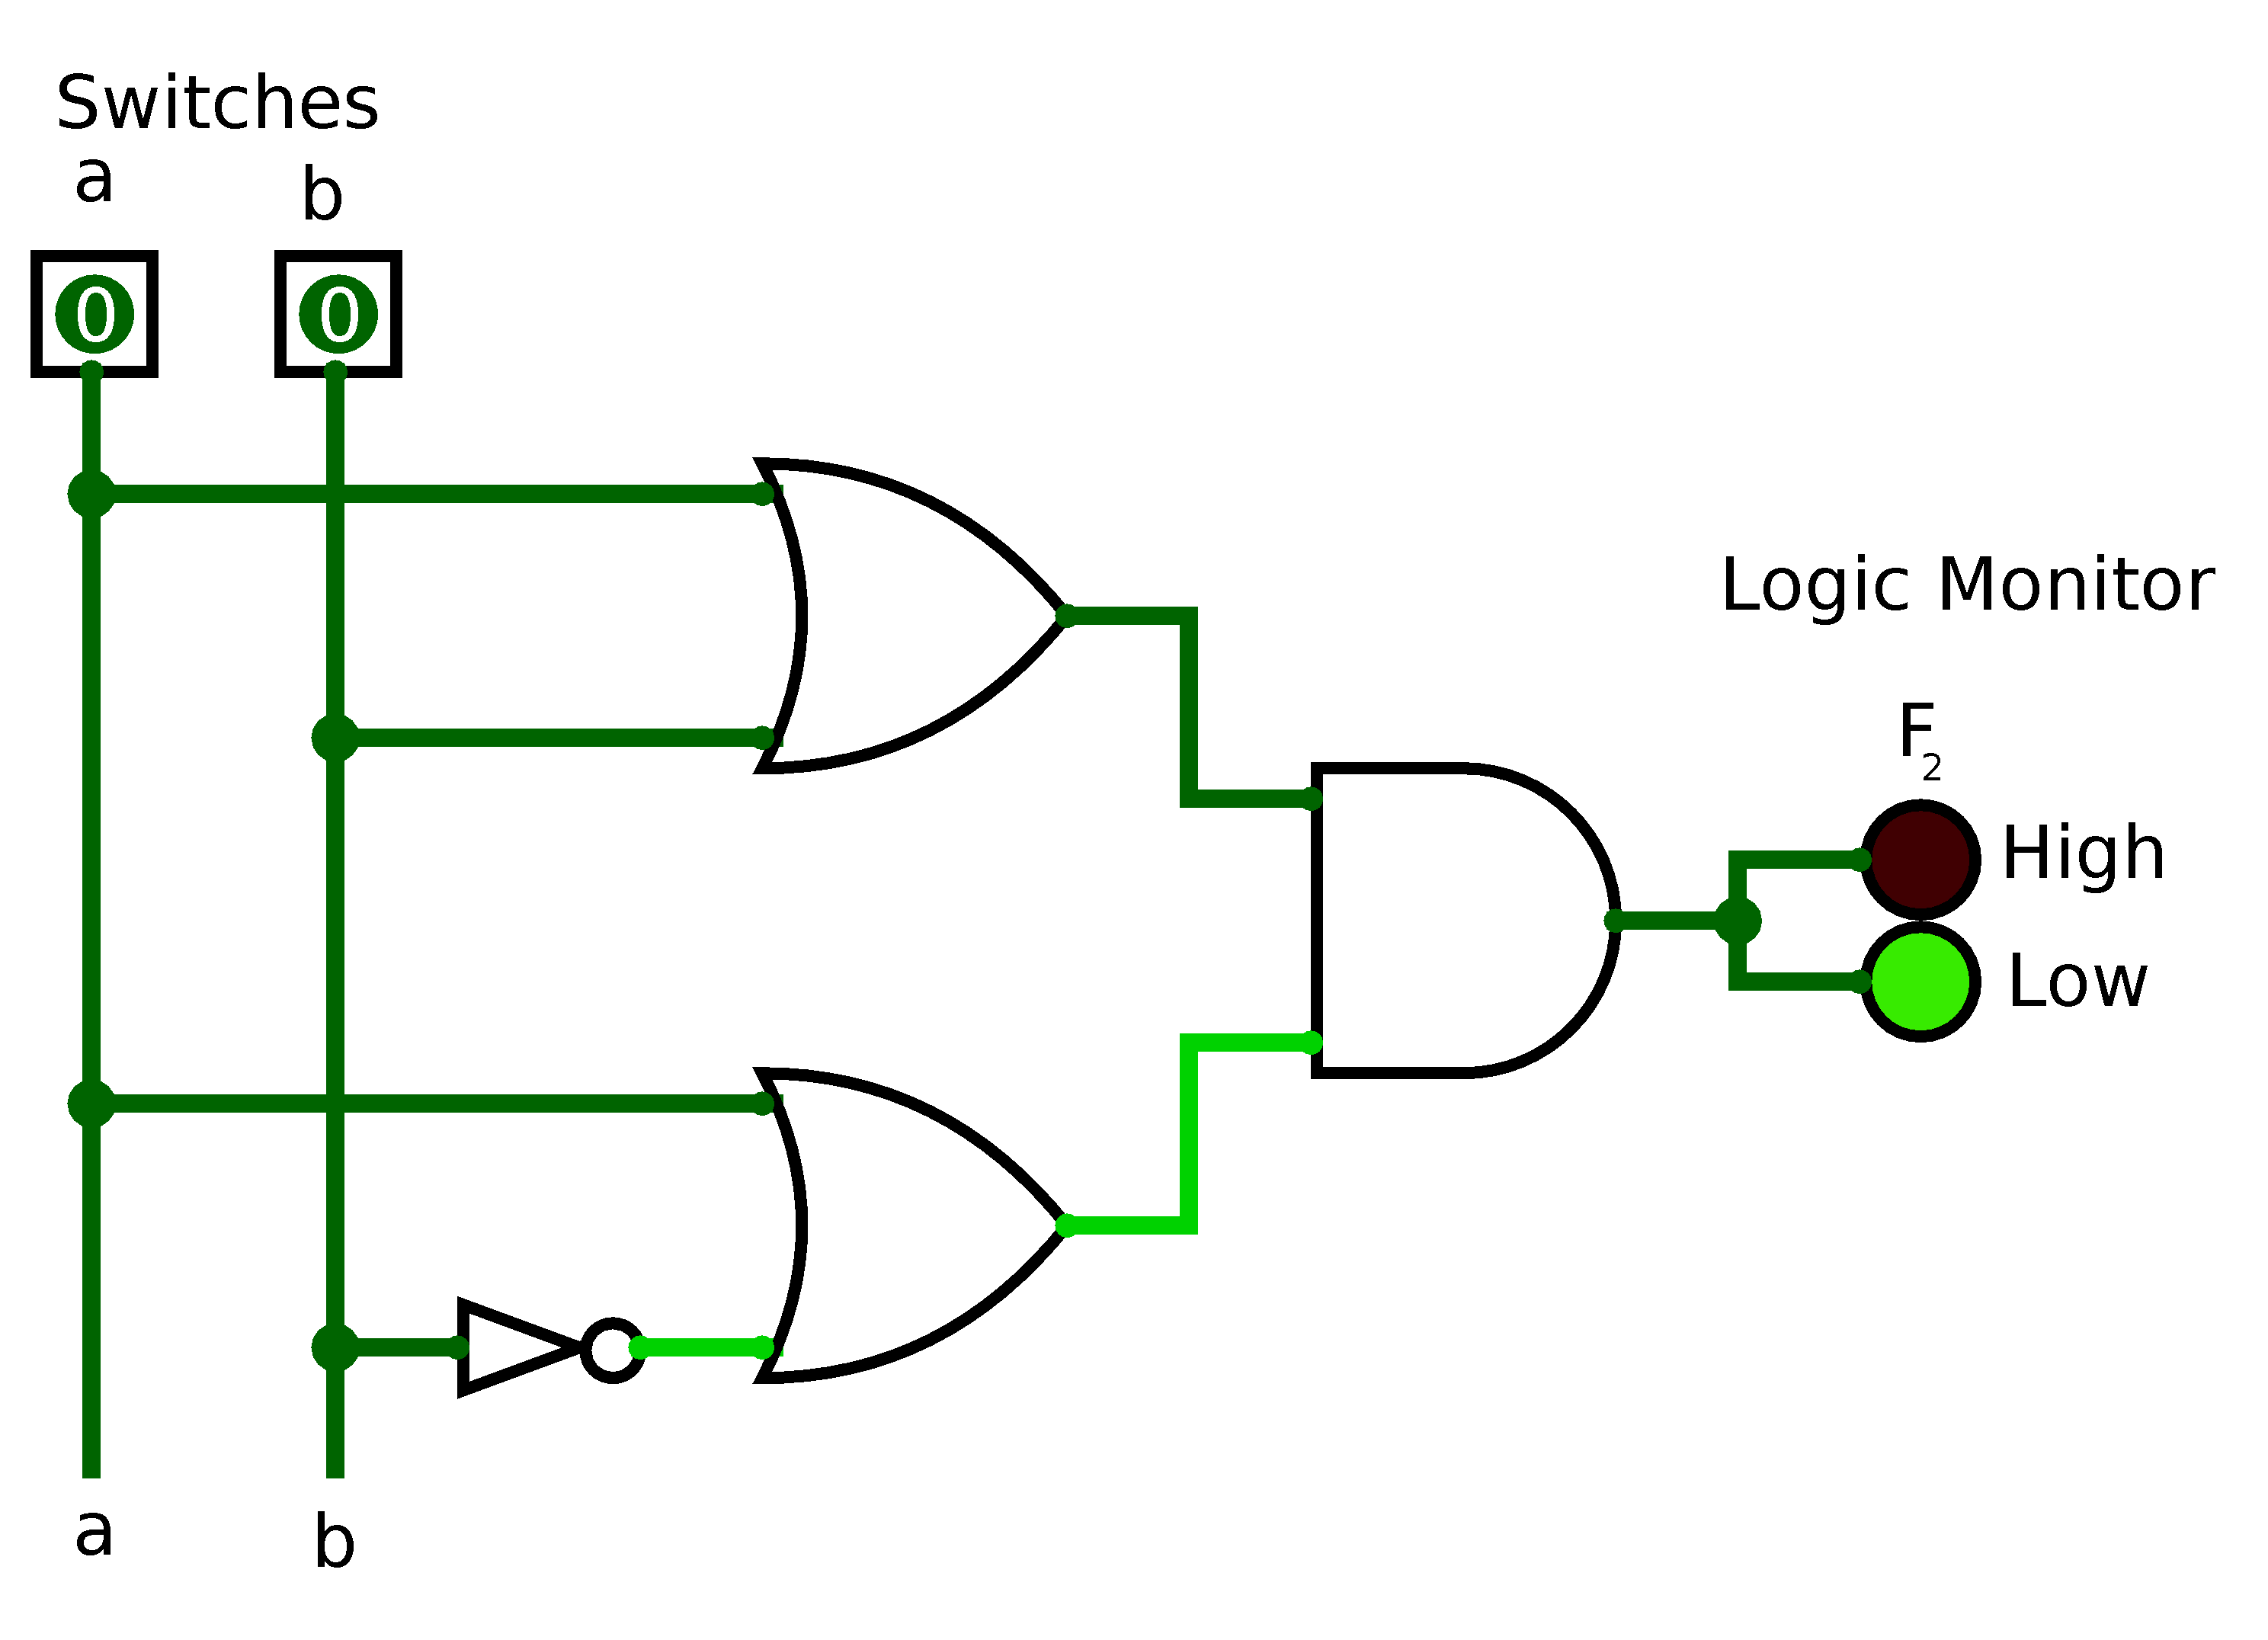
\includegraphics[width=0.5\textwidth]{part1-f2.png}	
	\caption{Circuit of $F_2$}
	\label{fig1}
\end{figure}
\begin{flushleft}

\end{flushleft}
\paragraph{}
In this part, hex inverter is used to invert the input value. 74x$x{1}$08 AND gate and 74x$x{1}$32 OR gate are used to implement necessary logic operations. The Vcc voltage is applied to the pins at the top right corner of each  integrated circuit and the ground voltage is applied to the pins at the lower left corner of each integrated circuit. 

\paragraph{}
To implement the first expression, the first input on the logic monitor(logic switches) is connected to the first pin on the left of the integrated circuit for OR operation. The first and second inputs on the logic monitor(logic switches) are connected to the first and second pin on the left of the integrated circuit for AND operation. The third pin on the left of integrated circuit for and operation, output value of AND operation, is connected to the second pin on the left of the integrated circuit for OR operation. The third pin on the left of the integrated circuit for OR operation is connected to the one of the pins on the logic monitor to observe output value.

\paragraph{}
For the second expression, the first input on the logic monitor(logic switches) is connected to the the first and fourth pin on the left of the integrated circuit for OR operation. The second input on the logic monitor is connected to the first pin on the left of the hex inverter and the second pin on the left of the integrated circuit for OR operation. The second pin on the left of hex inverter, output value of inverting operation, is connected to the fifth pin on the left of the integrated circuit for OR operation. The third and sixth pin on the left of the integrated circuit for OR operation is connected to the first and second pin on the left of the integrated circuit for AND operation. The third pin on the left of the integrated circuit for AND operation, output value of AND operation, is connected to the one of the pins on the logic monitor and output values are obs.rved
e\end{flushleft}

\begin{flushleft}
\subsection{PART 2}


\begin{figure}[!h]
	\centering
	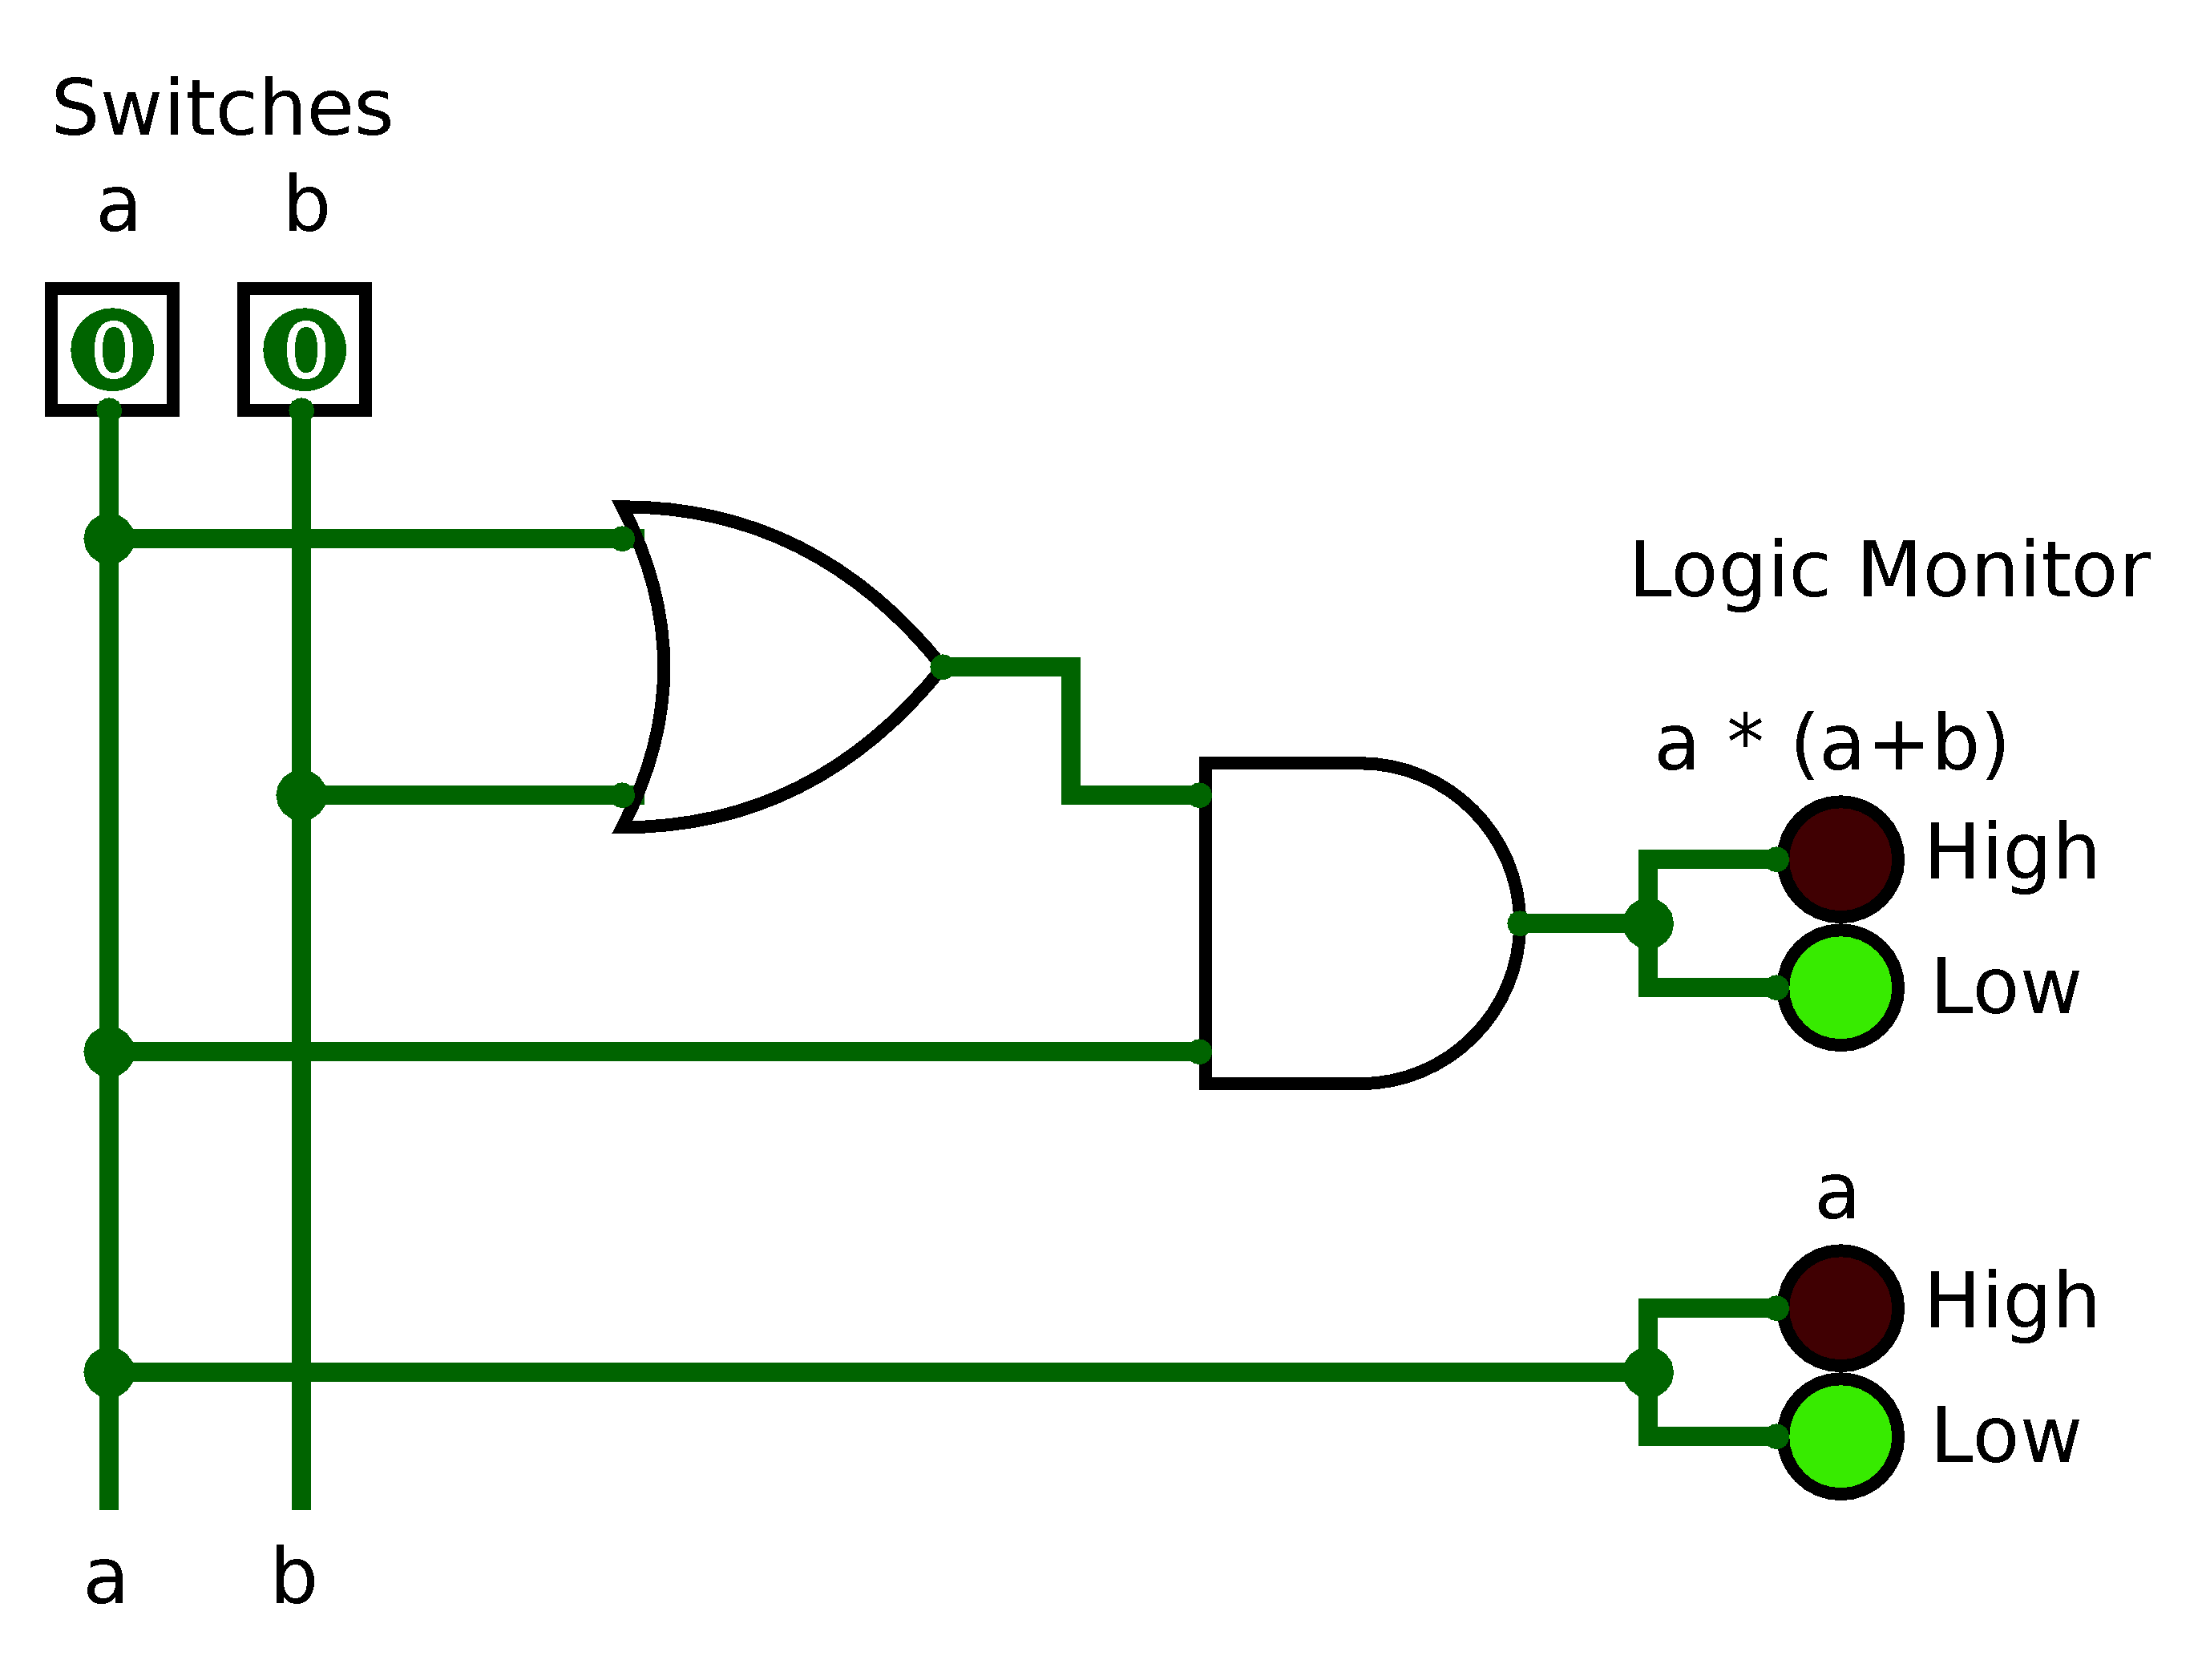
\includegraphics[width=0.5\textwidth]{part2.png}	
	\caption{Circuit of Part 2}
	\label{fig1}
\end{figure}

\paragraph{}
In the second part of the experiment, the logic circuit are designed and implemented for the dual of the expression below. At the end of the experiment it was shown that the expression's equal and its dual were equal. 

\begin{itemize}
    \item a + $a \cdot b$ = a
\end{itemize}

\paragraph{}
To find dual of the boolean expressions, AND's replace with OR's and OR's replace with AND's. Dual of the expression a + $a \cdot b$ = a is  shown below. 

\begin{itemize}
    \item $a \cdot (a + b)$ = a
\end{itemize}


\begin{table}[h]
    \centering
    \begin{tabular}{|c|c|c|c|c|c|}
    \hline
    a & b & b' & a + b & a + b' & $(a + b) \cdot (a + b')$ \\ \hline
    0 & 0 & 1  & 0     & 1      & 0                  \\
    0 & 1 & 0  & 1     & 0      & 0                  \\
    1 & 0 & 1  & 1     & 1      & 1                  \\
    1 & 1 & 0  & 1     & 1      & 1                  \\ \hline
    \end{tabular}
    \caption{Truth table of Part 2}
    \label{fig2}
\end{table}

% sadelestirme yontemleri ile yapmamiz lazim

% \begin{center}
% \begin{karnaugh-map}[4][4][1][c d][a b]
% \minterms{1,2,5,6,9,10,13,14}
% \autoterms[0]
% \implicant{1}{9}
% \implicant{2}{10}
% \end{karnaugh-map}
% \end{center}



\paragraph{}
In this part, 74x$x{1}$08 AND gate and 74x$x{1}$32 OR gate are used to implement necessary logic operations. The Vcc voltage is applied to the pins at the top right corner of each of the integrated circuits and the ground voltage is applied to the pins at the lower left corner. 

\paragraph{}
To implement the dual of the expression, the first input on the logic monitor(logic switches) connected to the first pin on the left of the integrated circuit for AND operation and the first pin on the left of the integrated circuit for OR operation. The second input of the logic monitor(logic switches) is connected to the second pin on the left of the logic monitor for OR operation. The third pin on the left of the integrated circuit for OR operation, output value of OR operation, is connected to the second pin on the left of the integrated circuit for AND operation. The third pin on the left of the integrated circuit for AND operation is connected to the one of the pins on the logic monitor and outpu
 tavule
 aesobserv d.re%TRUTH TABLE

\paragraph{}
When the table is examined, it can be seen that output value for the dual of the expression is equal to the output value of the expression itself.
\end{flushleft}

\begin{flushleft}
\subsection{PART 3}

\begin{figure}[!h]
	\centering
	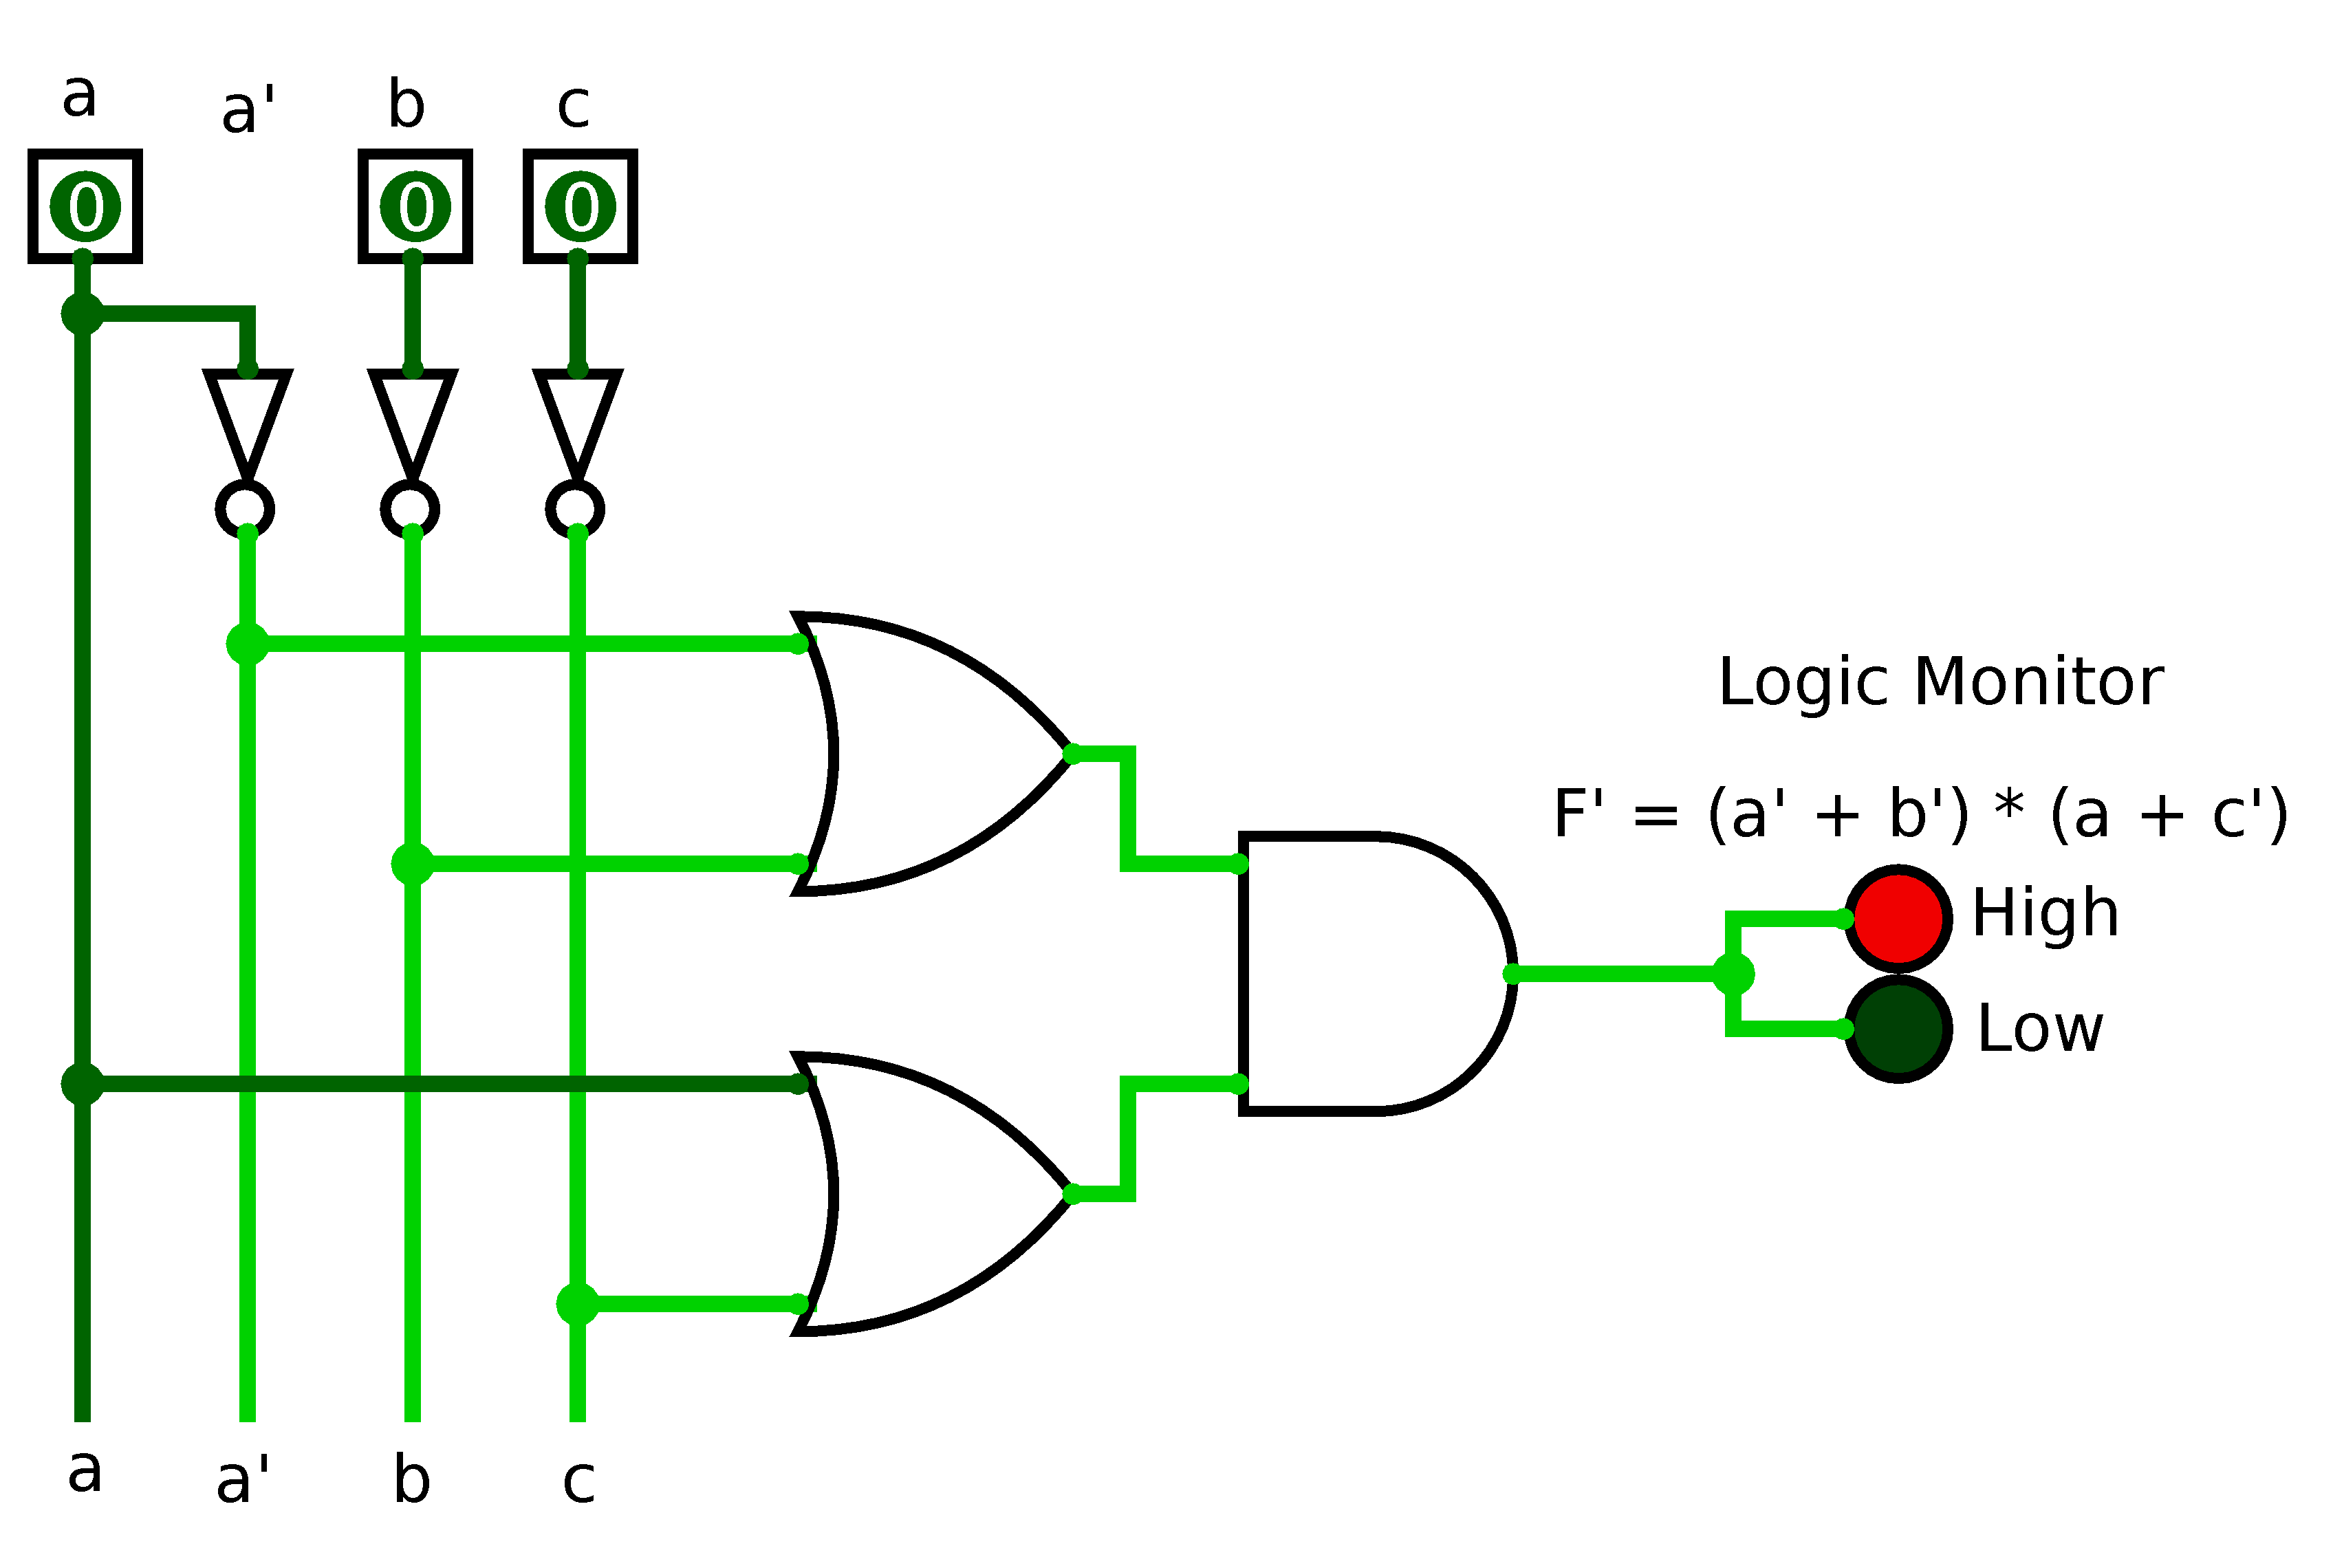
\includegraphics[width=0.5\textwidth]{part3.png}	
	\caption{Circuit for complement of F3}
	\label{fig1}
\end{figure}

\paragraph{}
In the third part of the experiment, the logic circuit are designed and implemented for the complement of the expression below. Then, truth table is found for the expression. At the end of this part it was validated that output values of the complementary function on the logic monitor is consistent with output values on the truth table.
\begin{itemize}
    \item $F_{3}$(a,b,c) = ($a \cdot b$) + ($a' \cdot b$)
\end{itemize}

\paragraph{}
To find the complement of any given boolean expressions AND's are replaced with OR's and OR's are replaced with AND's. Also, input variables are replaced with inverses of those variables. This way, complement of the expression above is found  as the expression below. 
\begin{itemize}
    \item F$'_{3}$(a,b,c) = $(a' + b') \cdot (a + c')$
\end{itemize}

\begin{table}[h]
\centering
\begin{tabular}{|c|c|c|c|c|c|c|c|}
\hline
a & b & c & a' & $a \cdot b$ & $a' \cdot c$ & $F_{3}$ = $a \cdot b$ + $a' \cdot c$ & $F'_{3}$ \\ \hline
0 & 0 & 0 & 1  & 0     & 0      & 0                        & 1        \\ 
0 & 0 & 1 & 1  & 0     & 1      & 1                        & 0        \\ 
0 & 1 & 0 & 1  & 0     & 0      & 0                        & 1        \\ 
0 & 1 & 1 & 1  & 0     & 1      & 1                        & 0        \\ 
1 & 0 & 0 & 0  & 0     & 0      & 0                        & 1        \\ 
1 & 0 & 1 & 0  & 0     & 0      & 0                        & 1        \\
1 & 1 & 0 & 0  & 1     & 0      & 1                        & 0        \\ 
1 & 1 & 1 & 0  & 1     & 0      & 1                        & 0        \\ \hline
\end{tabular}
\caption{Truth table for F3 and it's complement}
\label{fig3}
\end{table}

\paragraph{}
In this part, hex inverter is used to invert the input value. 74x$x{1}$08 AND gate and 74x$x{1}$32 OR gate are used to implement necessary logic operations. The Vcc voltage is applied to the pins at the top right corner of each of the integrated circuits and the ground voltage is applied to the pins at the lower left corner. 

\paragraph{}
To implement complement of the expression, the first input on the logic monitor(logic switch) is connected to the first pin on the left of the hex inverter and the fourth pin on the left of the integrated circuit for OR operation. The second pin on the left of the hex inverter is connected to the first pin on the left of the integrated circuit for OR operation. The second input on the logic monitor(logic switches) is connected to the third pin on the left of the hex inverter. The fourth pin on the left of the hex inverter is connected to the second pin of the integrated circuit for OR operation. The third input on the logic monitor is connected to the fifth pin on the left of the hex inverter. The sixth pin on the left of the hex inverter is connected to the fifth pin on the left of the integrated circuit for OR operation. The third and sixth pin on the left of the integrated circuit for OR operation are connected to the first and second pin on the left of the integrated circuit for AND operation. The third pin on the left of the integrated circuit for AND operation is connected to the one of the pins on the logic monitor to observe output value.

%TRUTH TABLE and Expreriment results

\paragraph{}
When the table is examined, it can be seen that output values of the expression on the truth table is consistent with output values on the logic monitor.
\end{flushleft}

\begin{flushleft}
\subsection{PART 4}

\begin{figure}[!h]
	\centering
	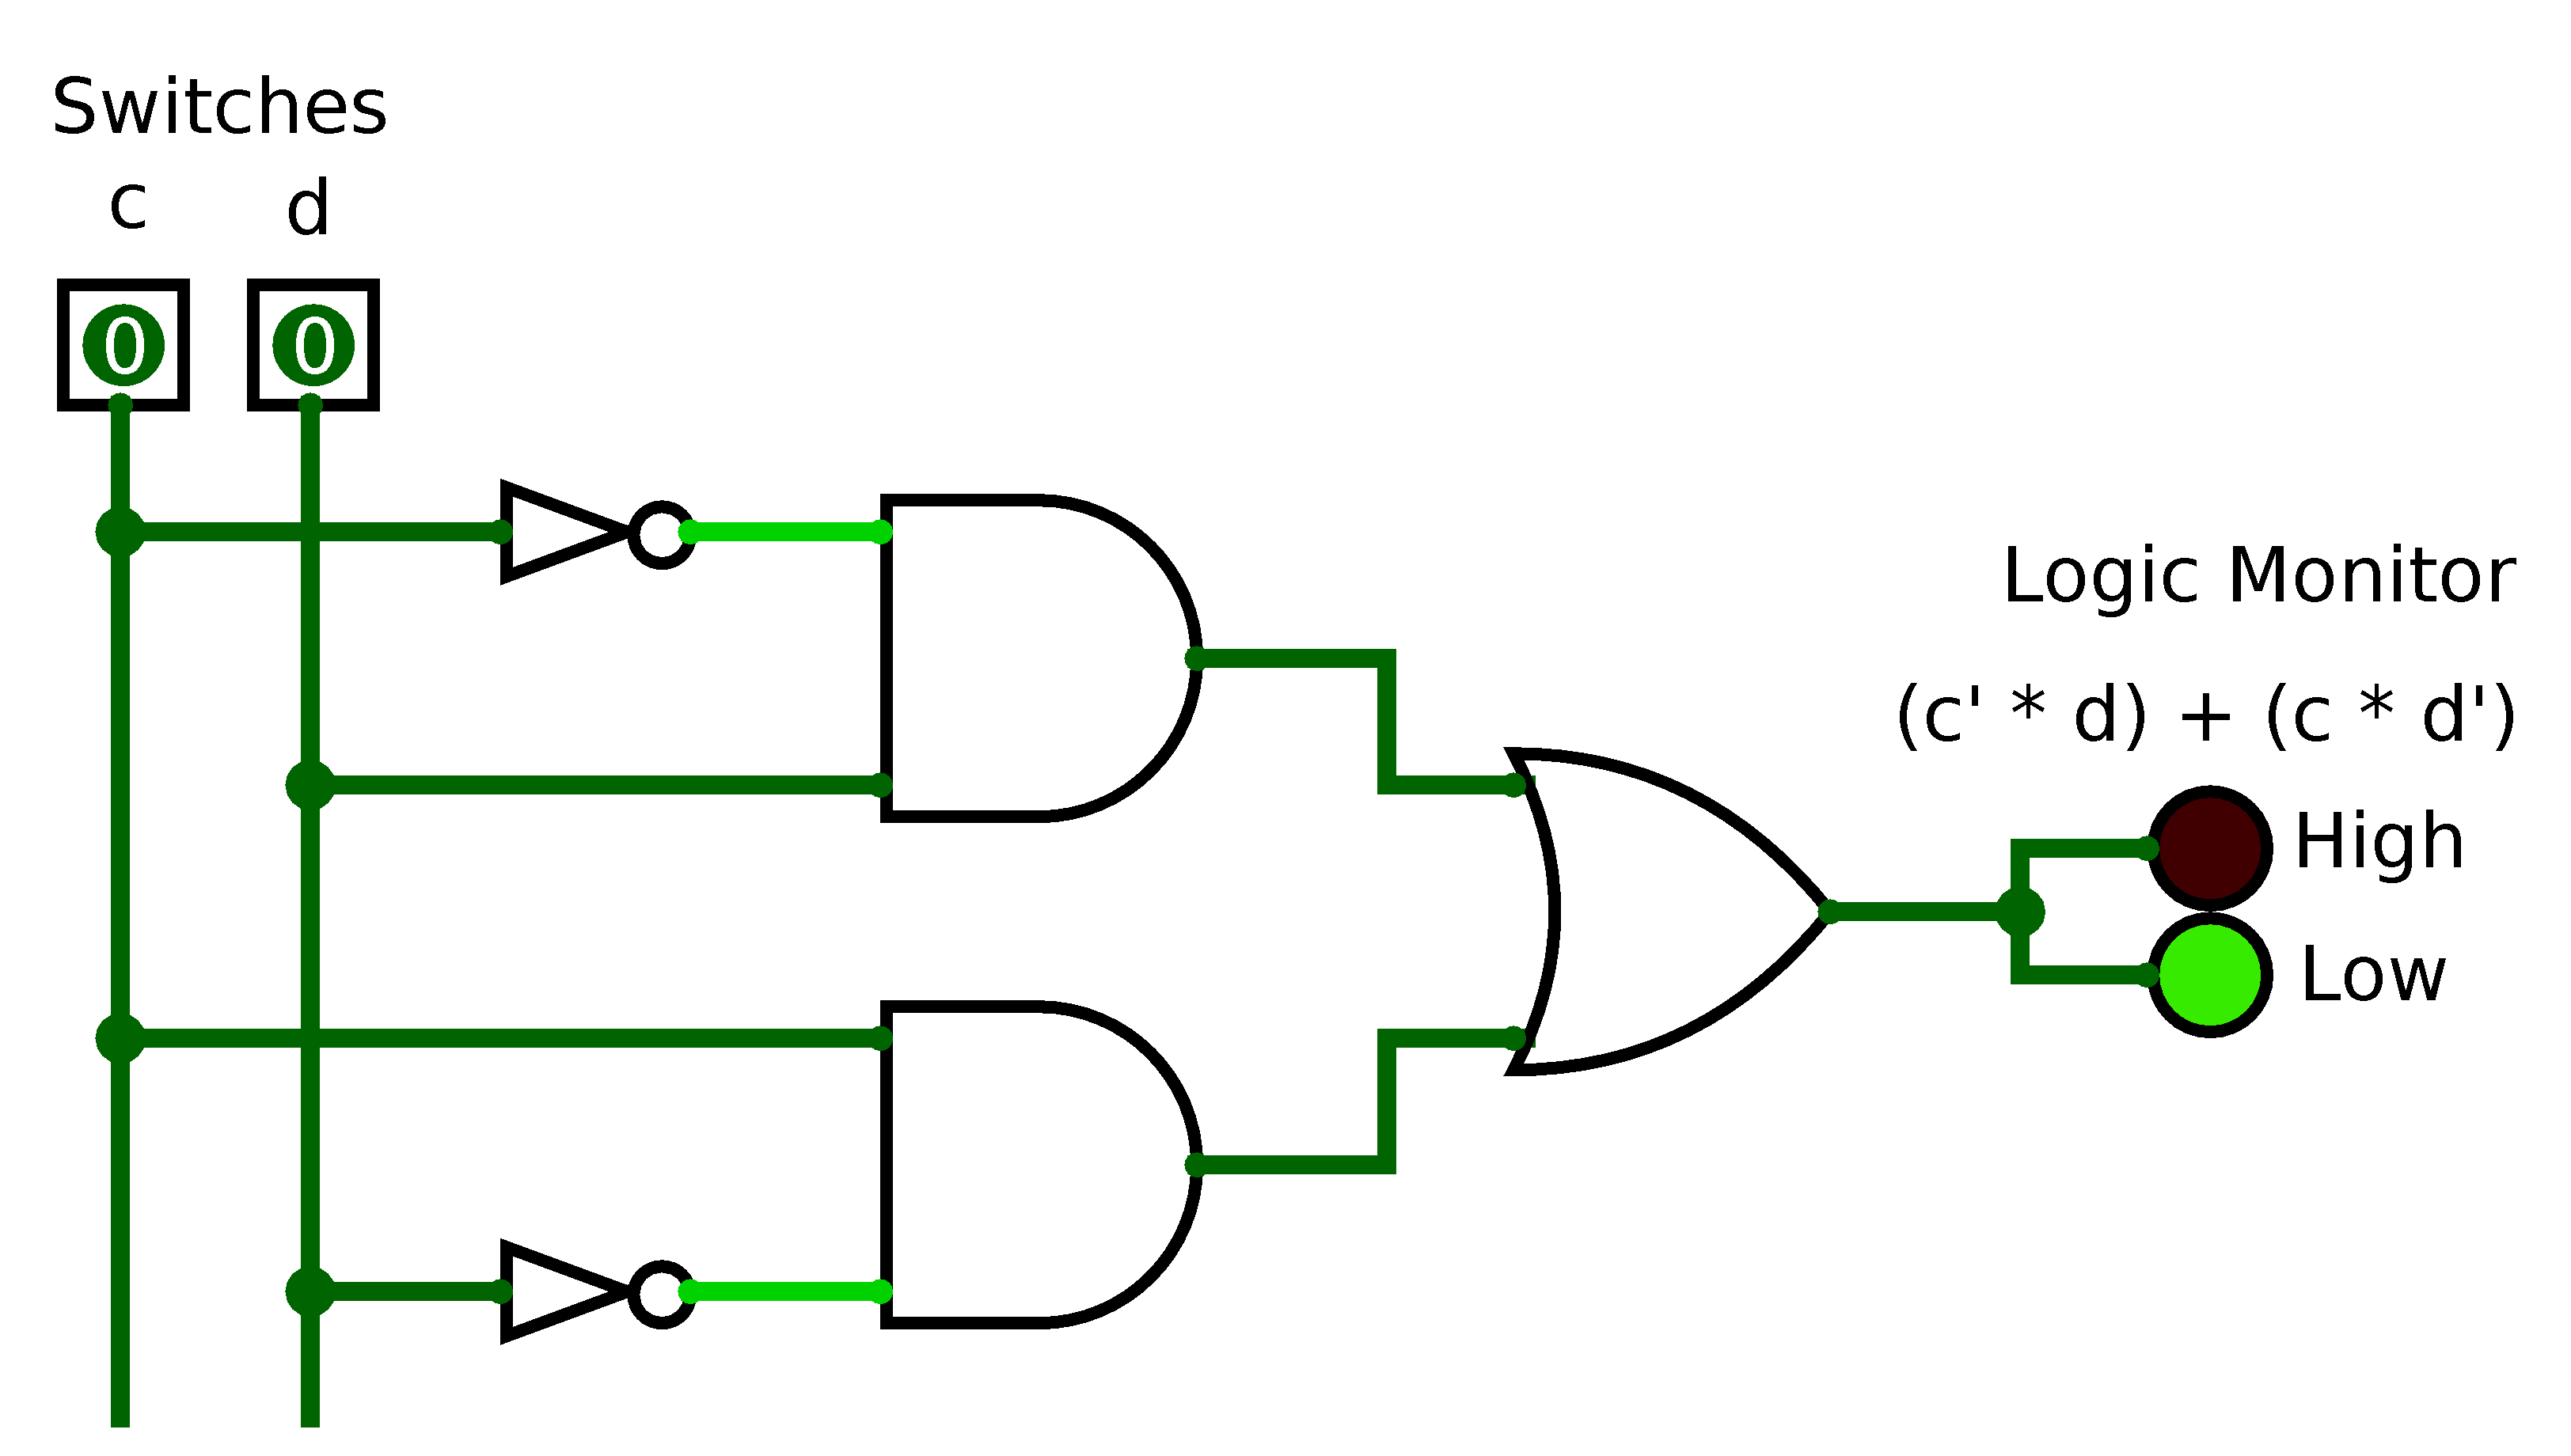
\includegraphics[width=0.5\textwidth]{part4.png}	
	\caption{Circuit of $F_4$}
	\label{fig1}
\end{figure}


\begin{table}[h]
\centering
\begin{tabular}{|c|c|c|c|c|c|c|c|c|}
\hline
a & b & c & d & c' & d' & $c' \cdot d$ & $c \cdot d'$ & $F_{4}$ = $c' \cdot d$ + $c \cdot d'$ \\ \hline
0 & 0 & 0 & 0 & 1  & 1  & 0      & 0      & 0                    \\ \hline
0 & 0 & 0 & 1 & 1  & 0  & 1      & 0      & 1                    \\ \hline
0 & 0 & 1 & 0 & 0  & 1  & 0      & 1      & 1                    \\ \hline
0 & 0 & 1 & 1 & 0  & 0  & 0      & 0      & 0                    \\ \hline
0 & 1 & 0 & 0 & 1  & 1  & 0      & 0      & 0                    \\ \hline
0 & 1 & 0 & 1 & 1  & 0  & 1      & 0      & 1                    \\ \hline
0 & 1 & 1 & 0 & 0  & 1  & 0      & 1      & 1                    \\ \hline
0 & 1 & 1 & 1 & 0  & 0  & 0      & 0      & 0                    \\ \hline
1 & 0 & 0 & 0 & 1  & 1  & 0      & 0      & 0                    \\ \hline
1 & 0 & 0 & 1 & 1  & 0  & 1      & 0      & 1                    \\ \hline
1 & 0 & 1 & 0 & 0  & 1  & 0      & 1      & 1                    \\ \hline
1 & 0 & 1 & 1 & 0  & 0  & 0      & 0      & 0                    \\ \hline
1 & 1 & 0 & 0 & 1  & 1  & 0      & 0      & 0                    \\ \hline
1 & 1 & 0 & 1 & 1  & 0  & 1      & 0      & 1                    \\ \hline
1 & 1 & 1 & 0 & 0  & 1  & 0      & 1      & 1                    \\ \hline
1 & 1 & 1 & 1 & 0  & 0  & 0      & 0      & 0                    \\ \hline
\end{tabular}
\caption{Thruth table for F4}
\label{fig3}
\end{table}

\paragraph{}
In the final part of the experiment, the logic circuit are designed and implemented for the basic logical expression below. 
\begin{itemize}
    \item $F_{4}$(a,b,c,d) = $U_{1}$(1,2,5,6,9,10,13,14)
\end{itemize}
\paragraph{}
If we write the minterms of of given function $F_{4}$ we obtain the first canonical form of $F_{4}$
\begin{itemize}
    \item $F_{4}(a,b,c,d) = (a' b'c' d) + (a' b'   c   d') + (a'   b   c'   d) + (a'   b   c   d') + (a   b'   c'   d) + (a   b'   c   d') + (a   b   c'   d) + (a   b   c'   d)$
\end{itemize}

\paragraph{}
To find simplified expression the axioms and theorems of Boolean algebra are used. 


\begin{align}
F_{4}(a,b,c,d) &= (a' b' c' d) + (a' b'   c   d') + (a'   b   c'   d) + (a'   b   c   d') + (a   b'   c'   d) + (a   b'   c   d') + (a   b   c'   d) + (a   b   c'   d) \notag\\ 
&= (a b' c' d) + (abc'd) + (a'b'cd') + (a'bcd') + (a'   b'   c'   d) + (a'   b   c'   d) + (a   b'   c   d') + (a   b   c   d') \tag{Commutativity} \\
&= ac'd(b' + b) + a'cd'(b'+b) + a'c'd(b' + b) + acd'(b'+b) \tag{Distribution} \\
&= ac'd(1) + a'cd'(1) + a'c'd(1) + acd'(1) \tag{Inverse} \\
&= ac'd + a'cd'+ a'c'd+ acd' \tag{Identitiy} \\
&= ac'd + a'c'd + a'cd' + acd' \tag{Commutativity} \\
&= c'd(a + a') + cd'(a' + a) \tag{Distribution} \\
&= c'd + cd' \notag
\end{align}

%%SIMPLFYING STEPS OF THE EXPRESSION


%%SIMPLIFIED FUNCTION
\begin{itemize}
    \item $F_{4}$(a,b,c,d) = ($c' \cdot d$) + ($c \cdot d'$)
\end{itemize}

\paragraph{}
In this part, hex inverter is used for inverting input value. 74x$x{1}$08 AND gate and 74x$x{1}$32 OR gate are used to implement necessary logic operations. The vcc voltage is applied to the pins at the top right corner of each of the integrated circuits and the ground voltage is applied to the pins at the lower left corner. 

\paragraph{}
To implement the minimized expression, the first input of the logic monitor is connected to the first pin on the left of the hex inverter and the fourth pin on the left of the integrated circuit for AND operation. The second pin on the left of the hex inverter is connected to the first pin on the left of the integrated circuit for AND operation. The second input of the logic monitor is connected to the third pin on the left of the hex inverter and the second pin on the left of the integrated circuit for AND operation. The fourth pin on the left of the hex inverter is connected to the fifth pin on the left of the integrated circuit for AND operation. The third and sixth pin on the left of the integrated circuit, output values of AND operations, are connected to the first and second pin on the left of the integrated circuit for OR operation. The third pin on the left of the integrated circuit for OR operation is connected to the one of the pins on the logic monitor the observe output value.


\paragraph{}
When the output values are observed, output values of the circuit that implemented with the minimized expression is consistent with the output values of the expression on the truth table. Thus, axioms and theorems of Boolean algebra are validated.

\end{flushleft}
\section{INTERPRETATION OF THE RESULTS}
\begin{flushleft}
\paragraph{}
Throughout the whole experiment results we observed were consistent with the theoretical results. Since all operations
 were logical operations there were no swings in voltage values that would cause us to get wrong result (Also no equipment failures occured).
\end{flushleft}

\section{CONCLUSION}
\begin{flushleft}
\paragraph{}For the most part we were able to go through each part without any big problems. Only issue worth mentioning was a confusion we had while plugging the cables for the last part of the experiment. Which resulted in us getting wrong logic results from the circuit. But we figured it out and corrected it rather quickly. We have seen that a little more care has to be taken while assembling the circuits in order not to make a mistake and be more efficient with time.
\end{flushleft}

\nocite{overleaf}
\nocite{reportGuide}

\newpage


\addcontentsline{toc}{section}{\numberline {}REFERENCES}

\bibliographystyle{unsrt}
\bibliography{reference}

\end{document}

